\chapter{Результаты}

В этой главе приведены результаты спектрального анализа промежуточных представлений моделей ResNet, ViT и Swin. Я отдельно рассматриваю два типа материалов: радиальные спектральные кривые и сводные численные метрики, рассчитанные по этим кривым. Такой порядок нужен для того, чтобы сначала увидеть форму спектра визуально, а затем проверить те же наблюдения через центроид, долю низкочастотной энергии и скорость спектрального сжатия.

\section{Спектральные кривые}

\subsection{Динамика внутри ResNet}

На Рис. \ref{fig:ResNet18} показано, как меняется радиальный спектр мощности при переходе от layer1 к layer4 в ResNet18. Здесь хорошо видна типичная для CNN картина: ранний уровень даёт более широкий спектр, а поздние уровни постепенно стягивают энергию к области малых частотных радиусов. У layer1 хвост кривой длиннее. Это значит, что в представлении ещё остаётся заметная доля средне- и высокочастотных компонент, связанных с границами, текстурами и мелкими локальными изменениями.

Дальше спектр становится уже. На layer2 и layer3 вклад высоких частот уменьшается, а на layer4 кривая занимает уже довольно ограниченный участок частотной оси. По сути, слой всё меньше похож на представление с большим количеством локальных деталей и всё больше — на сглаженное описание более крупных структур. Для ResNet это ожидаемо: при переходе между стадиями уменьшается пространственное разрешение, растёт рецептивное поле, а признаки становятся более агрегированными.

ResNet18 на этом графике даёт удобный базовый пример спектрального сжатия в свёрточной сети. Ранние карты признаков ещё сохраняют широкий частотный диапазон, поздние — переходят к низкочастотному описанию. В терминах данной работы это означает постепенное подавление пространственно мелких компонент по мере продвижения к финальным блокам.

\begin{figure}[h]
    \centering % Центрируем изображение
    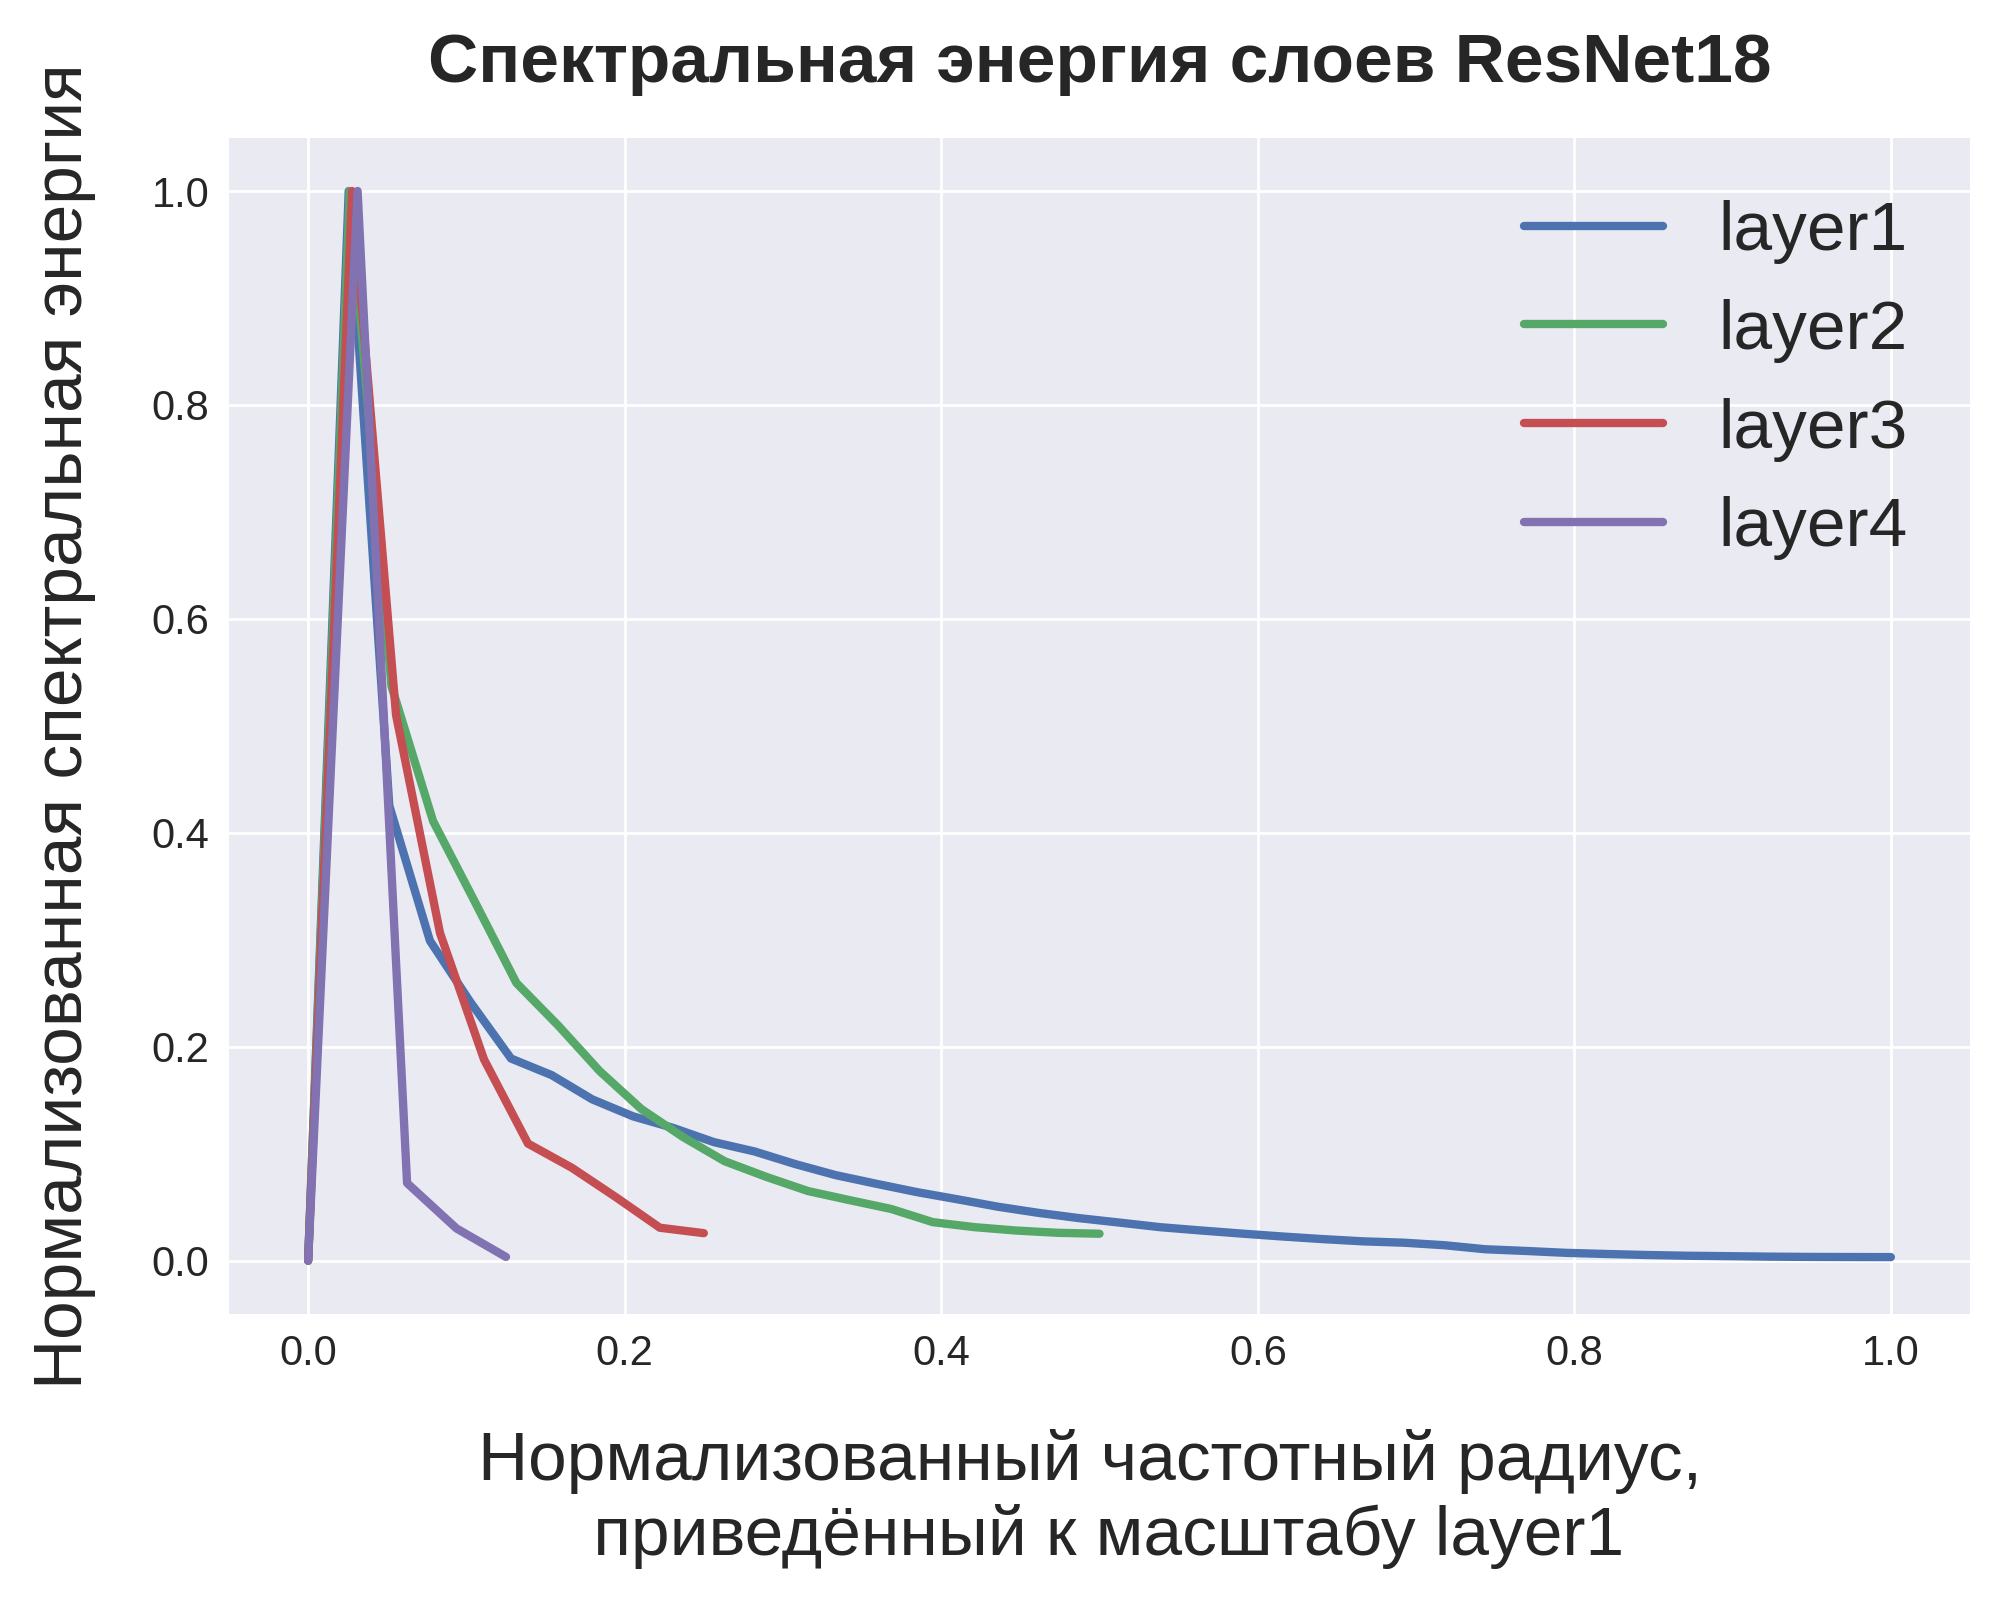
\includegraphics[width=0.8\textwidth]{images/compare/ResNet18.png} % Масштабируем до 80% ширины текста
    \caption{Изменение спектрального профиля по слоям ResNet18.} % Подпись
    \label{fig:ResNet18} % Метка для ссылки в тексте
\end{figure}

На Рис. \ref{fig:resnet_last_block} сравниваются спектры последнего блока у ResNet18, ResNet34, ResNet50 и ResNet101. Общая форма у всех моделей близкая: максимум находится в низкочастотной области, а доступный частотный диапазон после приведения к масштабу layer1 заметно ограничен. Значит, финальные представления всех вариантов ResNet имеют выраженный низкочастотный характер.

Различия между моделями всё же есть. У ResNet50 и ResNet101 хвост немного заметнее, чем у ResNet18 и ResNet34. Это согласуется с таблицей спектрального центроида: финальные значения у ResNet50/101 чуть выше, чем у ResNet18/34 (Таб. \ref{tab:SpectraCentr_metrics}). Но это различие не меняет основную картину. Внутри семейства ResNet глубина влияет на детали формы кривой, а не на сам тип финального спектрального профиля.

\begin{figure}[h]
    \centering % Центрируем изображение
    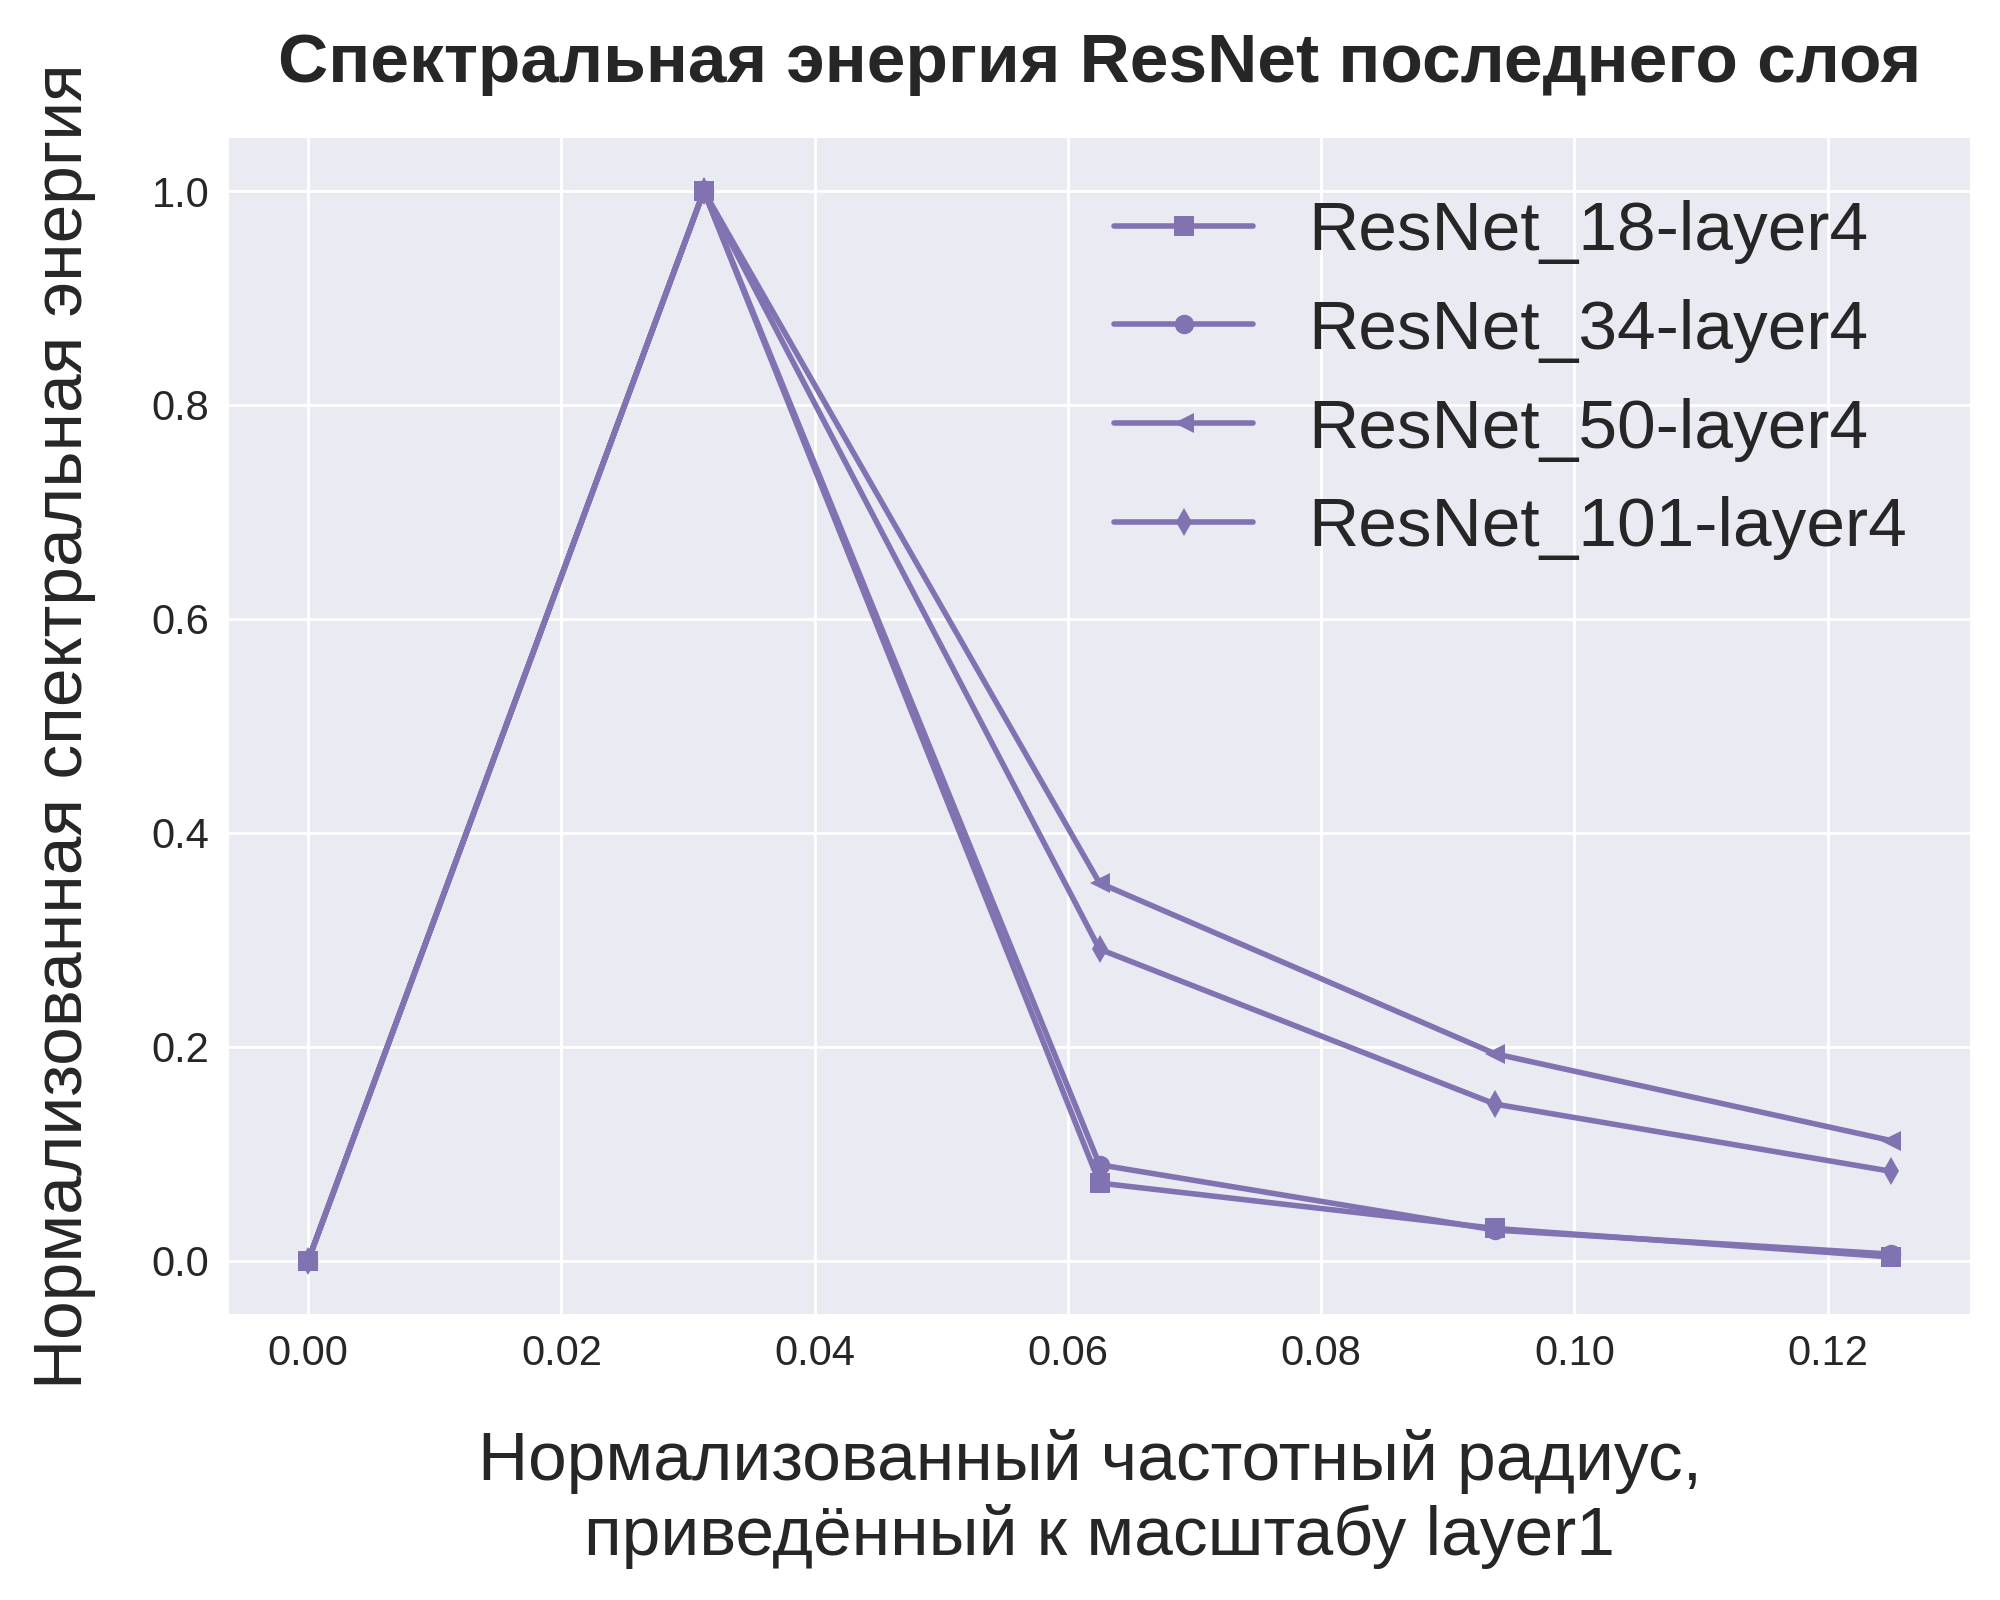
\includegraphics[width=0.8\textwidth]{images/compare/resnet_last_block.png} % Масштабируем до 80% ширины текста
    \caption{Сравнение спектров последних слоёв ResNet разной глубины.} % Подпись
    \label{fig:resnet_last_block} % Метка для ссылки в тексте
\end{figure}

\subsection{Динамика внутри ViT}

На Рис. \ref{fig:vit_l_16_imagenet_spectra} приведены спектральные кривые выбранных блоков ViT-L/16. По сравнению с ResNet поведение здесь другое. Не видно простого движения, при котором каждый следующий блок всё сильнее сжимает спектр к низким частотам. Напротив, поздние блоки ViT-L/16 сохраняют более длинный хвост в области средних и высоких частот. Особенно заметны block\_18 и block\_23: спад у них более пологий, а энергия на больших частотных радиусах остаётся заметной.

\begin{figure}[h]
    \centering % Центрируем изображение
    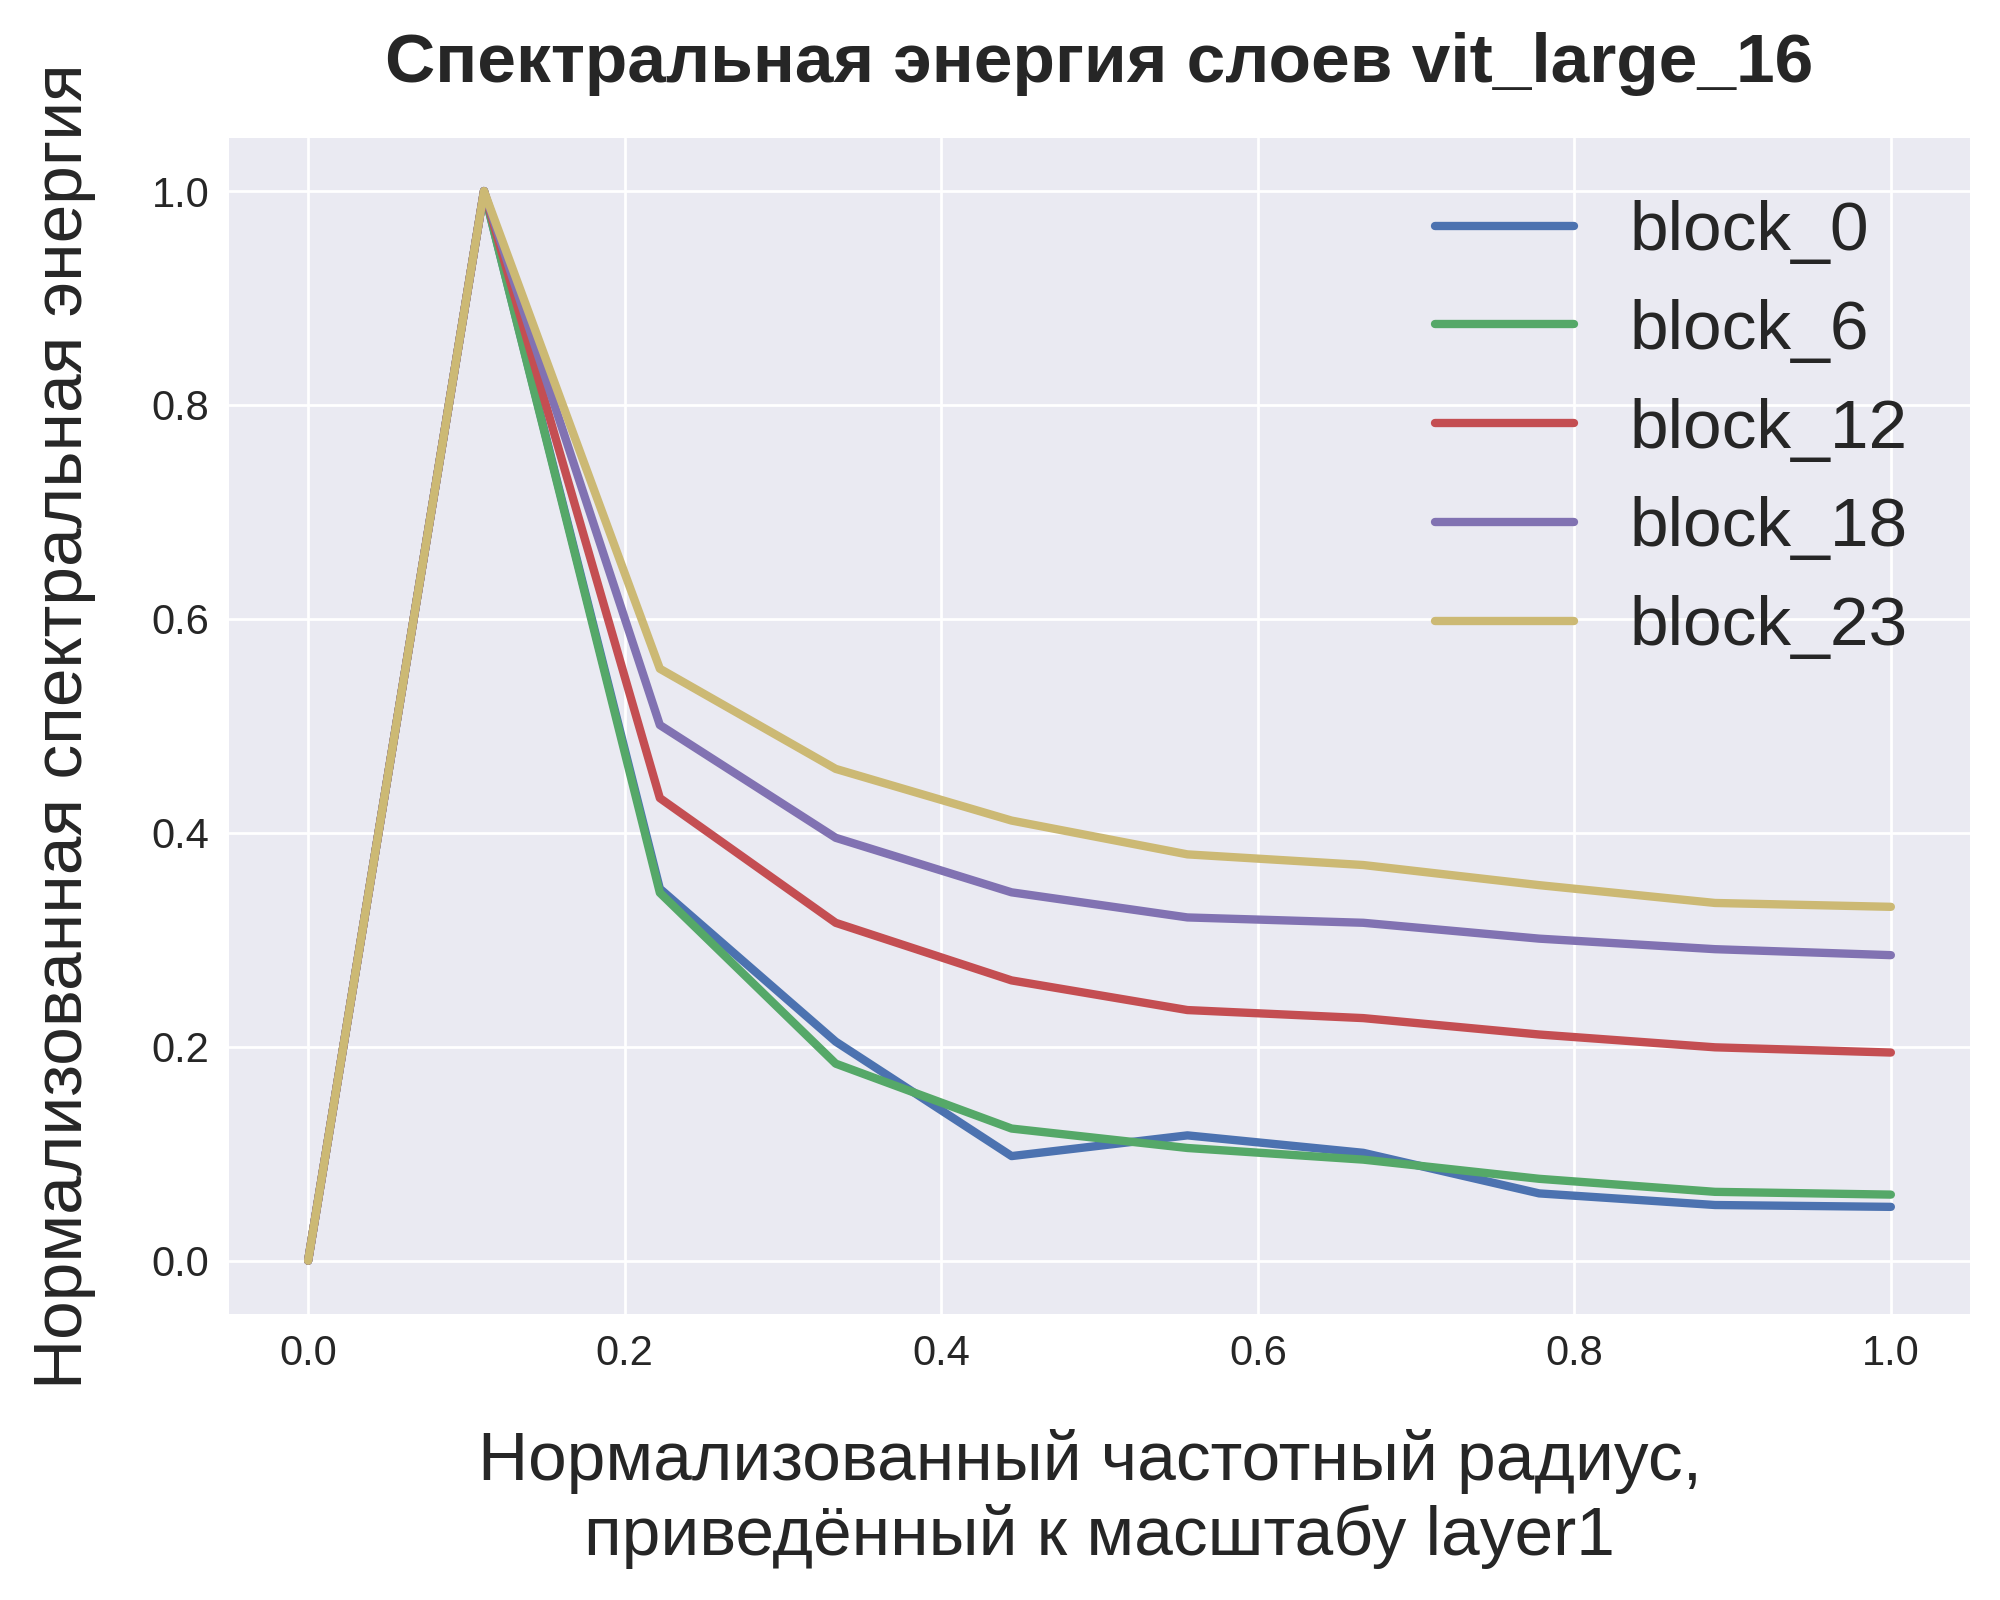
\includegraphics[width=0.8\textwidth]{images/compare/vit_l_16_imagenet_spectra.png} % Масштабируем до 80% ширины текста
    \caption{Изменение спектрального профиля по блокам ViT-L/16.} % Подпись
    \label{fig:vit_l_16_imagenet_spectra} % Метка для ссылки в тексте
\end{figure}

Причина такого отличия связана с устройством ViT. В ResNet пространственное разрешение уменьшается от стадии к стадии, и вместе с этим сужается набор частот, которые карта признаков может нести. В ViT последовательность патчей проходит через блоки при неизменной решётке. Преобразование задаётся вниманием, MLP-блоками и остаточными соединениями. Поэтому часть блоков может не только сглаживать токенные представления, но и усиливать различия между патчами.

Более широкий спектр на поздних блоках не стоит читать как прямое доказательство лучшего сохранения полезной семантики. График говорит о другом: в выбранном протоколе ViT-L/16 остаётся менее жёстко сжатым к низким частотам, чем CNN-представления. Что именно несёт эта энергия — полезные детали, особенности токенного кодирования или побочные вариации, — требует отдельной проверки. В рамках этой работы фиксируется сам факт: динамика ViT не похожа на последовательное подавление высоких частот.

Сравнение последних блоков моделей ViT (модификации Tiny, Small, Base и Large) представлено на Рис. \ref{fig:vit_block_last}. В отличие от ResNet, на финальном слое расхождения между этими конфигурациями становятся более очевидными. Для модели ViT-Large характерно наличие более протяженного «хвоста» на графике распределения, а также удержание большего объема относительной энергии в диапазоне средних частот.

\begin{figure}[h]
    \centering % Центрируем изображение
    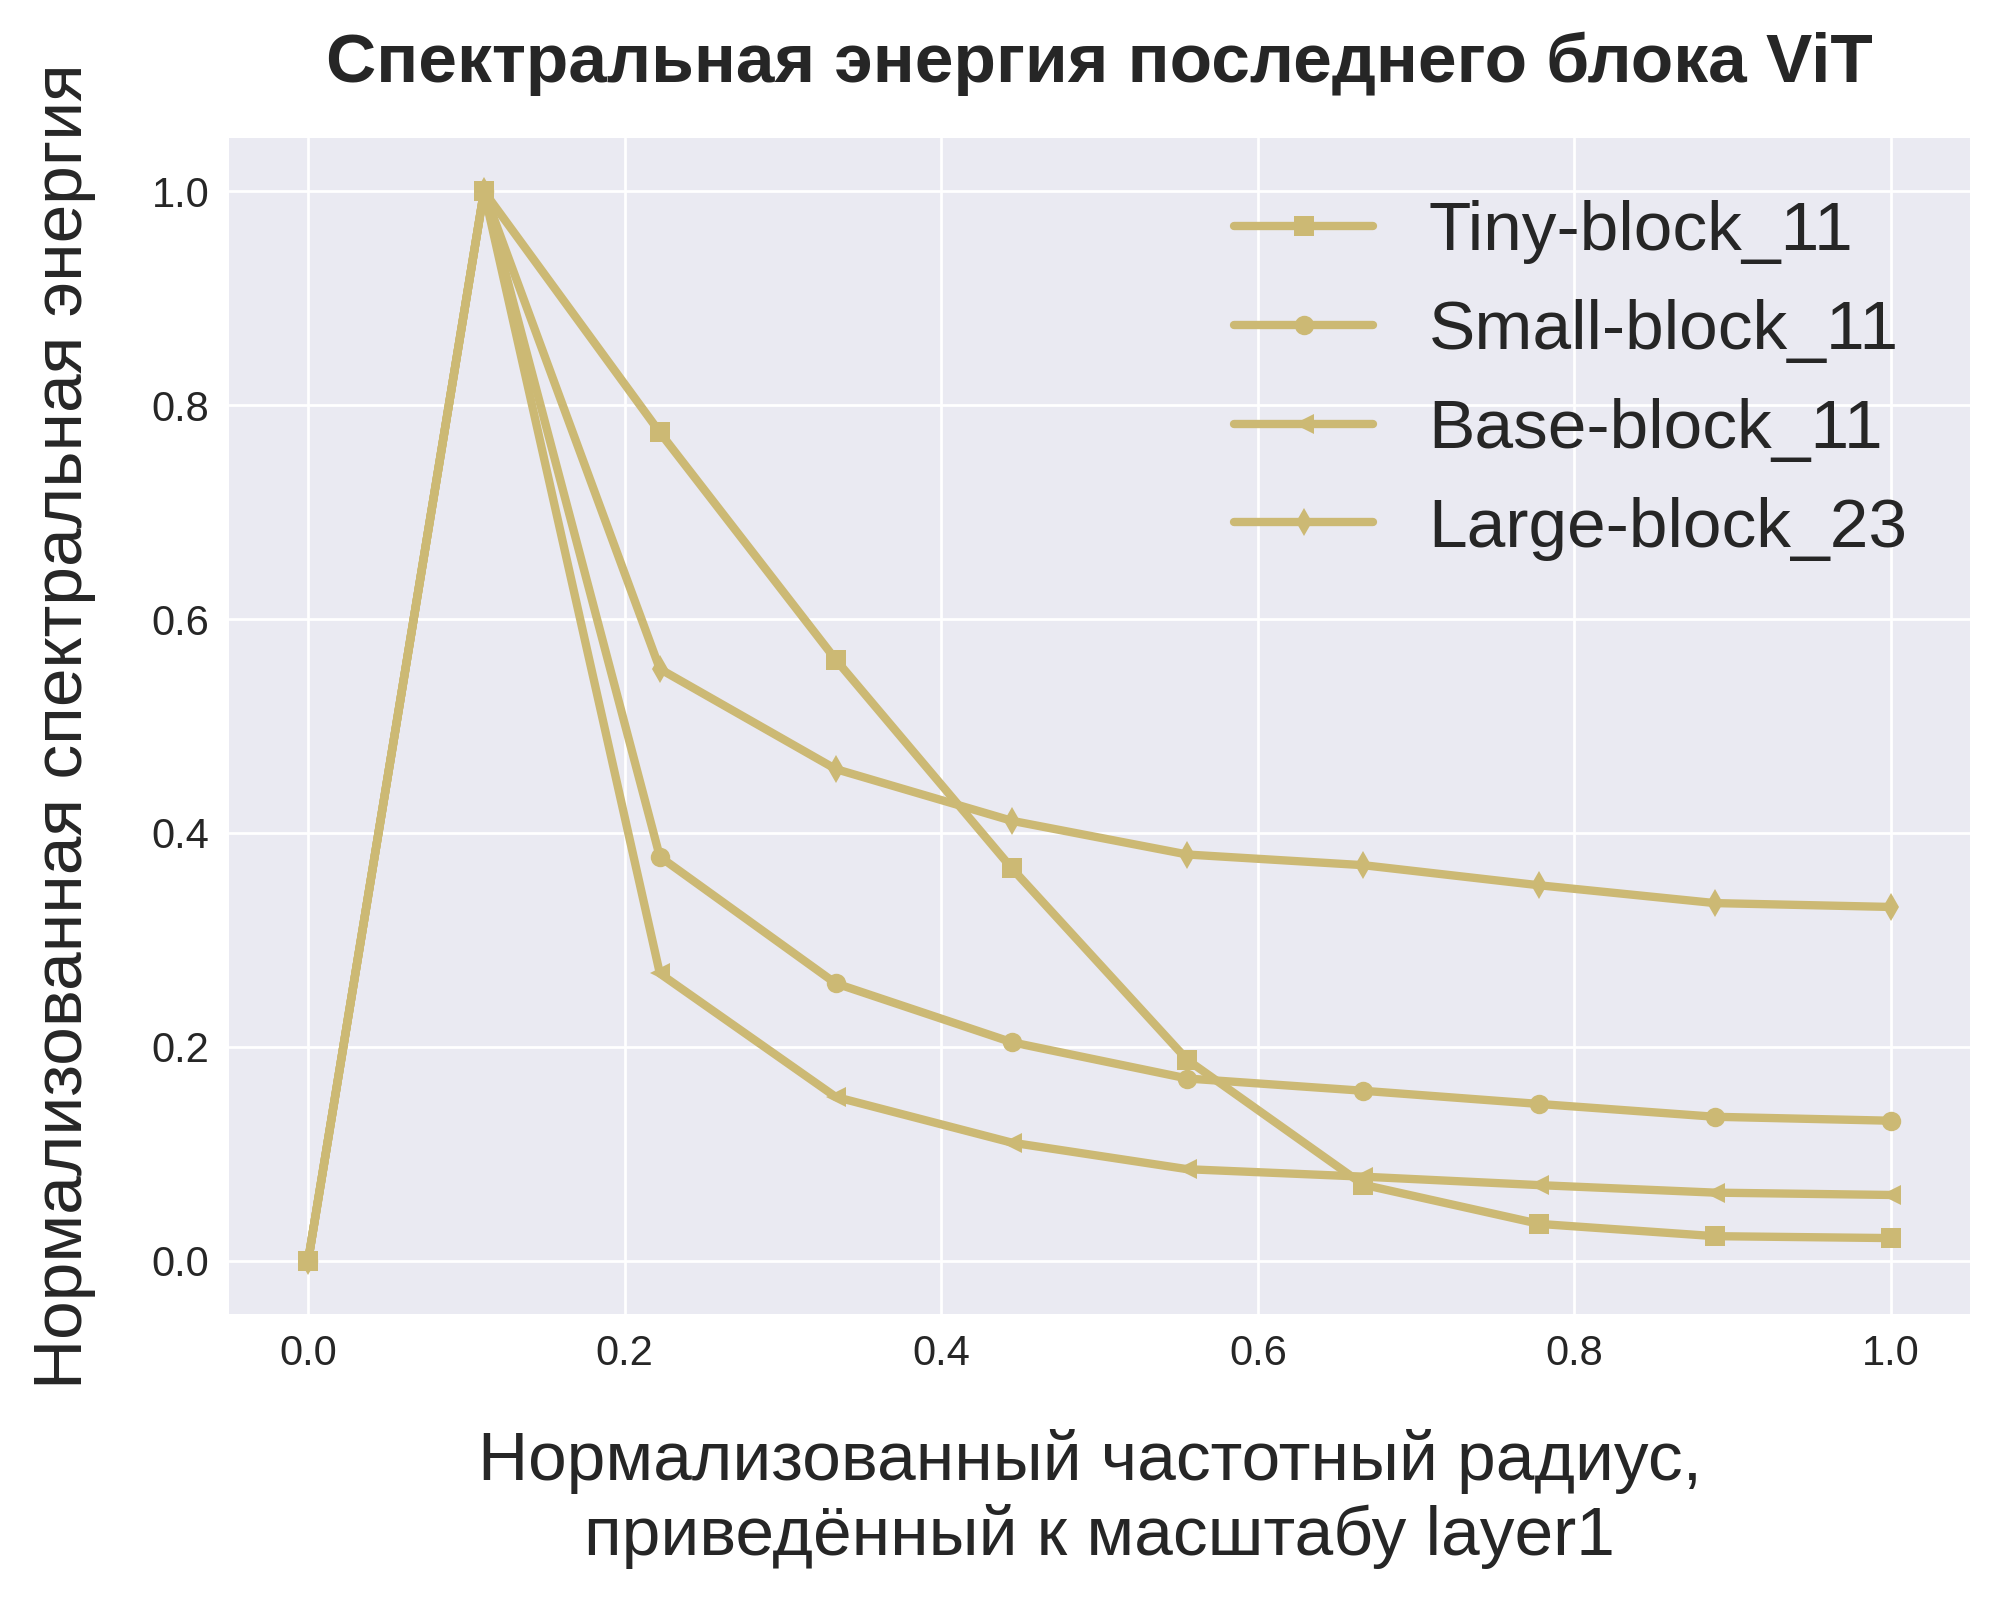
\includegraphics[width=0.8\textwidth]{images/compare/vit_block_last.png} % Масштабируем до 80% ширины текста
    \caption{Сравнение спектров последних слоёв ViT разного масштаба.} % Подпись
    \label{fig:vit_block_last} % Метка для ссылки в тексте
\end{figure}

На этом сравнении видно, что масштаб ViT отражается не только на числе параметров. Меняется и сам вид финального спектра. В данном эксперименте более крупная модель не приходит к более узкому низкочастотному профилю. Напротив, ViT-Large сохраняет более протяжённый хвост; это согласуется с повышенным центроидом large-модели в Таб. \ref{tab:SpectraCentr_metrics}. Поэтому внутри семейства ViT размер модели связан и с формой финального представления, а не только с вычислительной мощностью.

\subsection{Динамика внутри Swin}

На Рис. \ref{fig:swin_base} показана динамика выбранных блоков Swin-Base. Начальный блок даёт резкий пик около низких частот и сравнительно быстрый спад. Это похоже на сильную локальную агрегацию уже на раннем этапе обработки. Но далее картина не остаётся полностью простой: на промежуточных стадиях некоторые блоки имеют более широкий хвост и сохраняют заметную энергию в области средних частот. Вероятное объяснение — работа shifted window attention, где локальные окна чередуются со сдвинутыми окнами и дают обмен информацией между соседними областями изображения.

Поздний блок снова выглядит более низкочастотным. После перехода к последней иерархической стадии Swin приходит к более узкому спектральному диапазону, но путь к этому состоянию не повторяет ResNet один к одному. Swin здесь лучше описывать как архитектуру со смешанной динамикой: patch merging тянет представления к CNN-подобному сжатию, а оконное внимание даёт промежуточные перераспределения энергии.

\begin{figure}[h]
    \centering % Центрируем изображение
    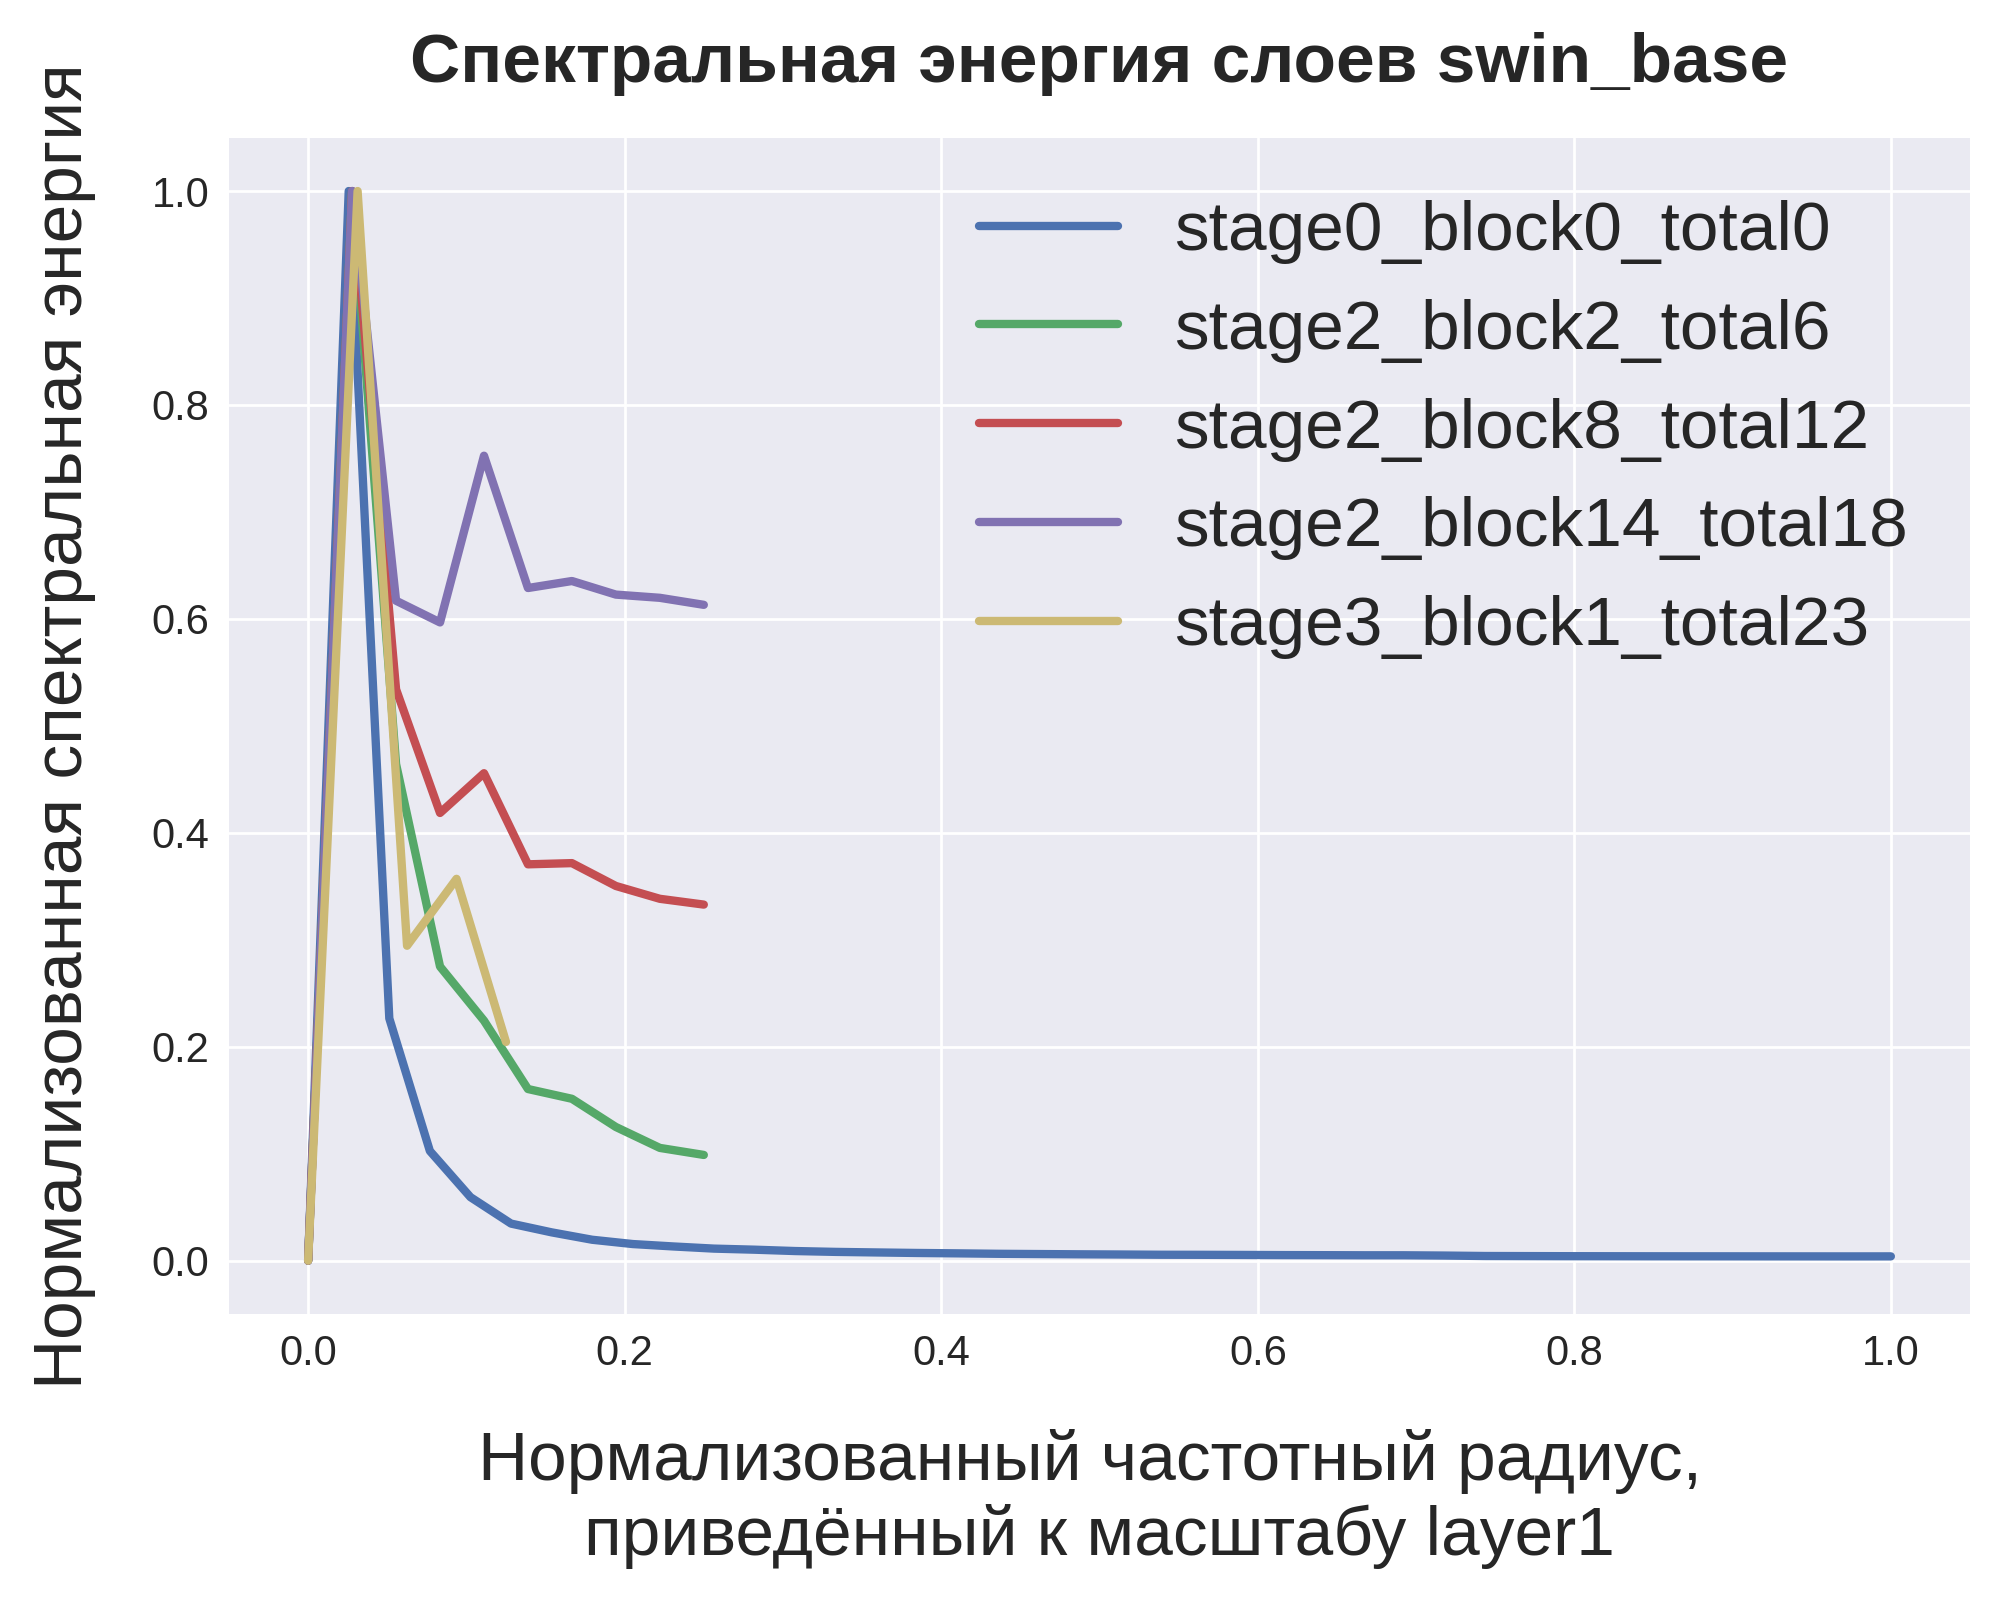
\includegraphics[width=0.8\textwidth]{images/compare/swin_base.png} % Масштабируем до 80% ширины текста
    \caption{Изменение спектрального профиля по блокам Swin-Base.} % Подпись
    \label{fig:swin_base} % Метка для ссылки в тексте
\end{figure}

На Рис. \ref{fig:swin_block_last} представлены спектры последних блоков Swin-Tiny, Swin-Small, Swin-Base и Swin-Large. Все кривые имеют общий максимум в низкочастотной области и достаточно близкую форму. Это отличает Swin от ViT: у ViT финальные спектры разных масштабов расходятся сильнее.

У Swin финальная стадия, судя по графику, стабилизируется архитектурной иерархией. Независимо от размера модели последние блоки приходят к сходному низкочастотному профилю. Локальное оконное внимание и объединение патчей не делают Swin обычной CNN, но в финальных представлениях они дают близкое направление спектрального сжатия.

\begin{figure}[h]
    \centering % Центрируем изображение
    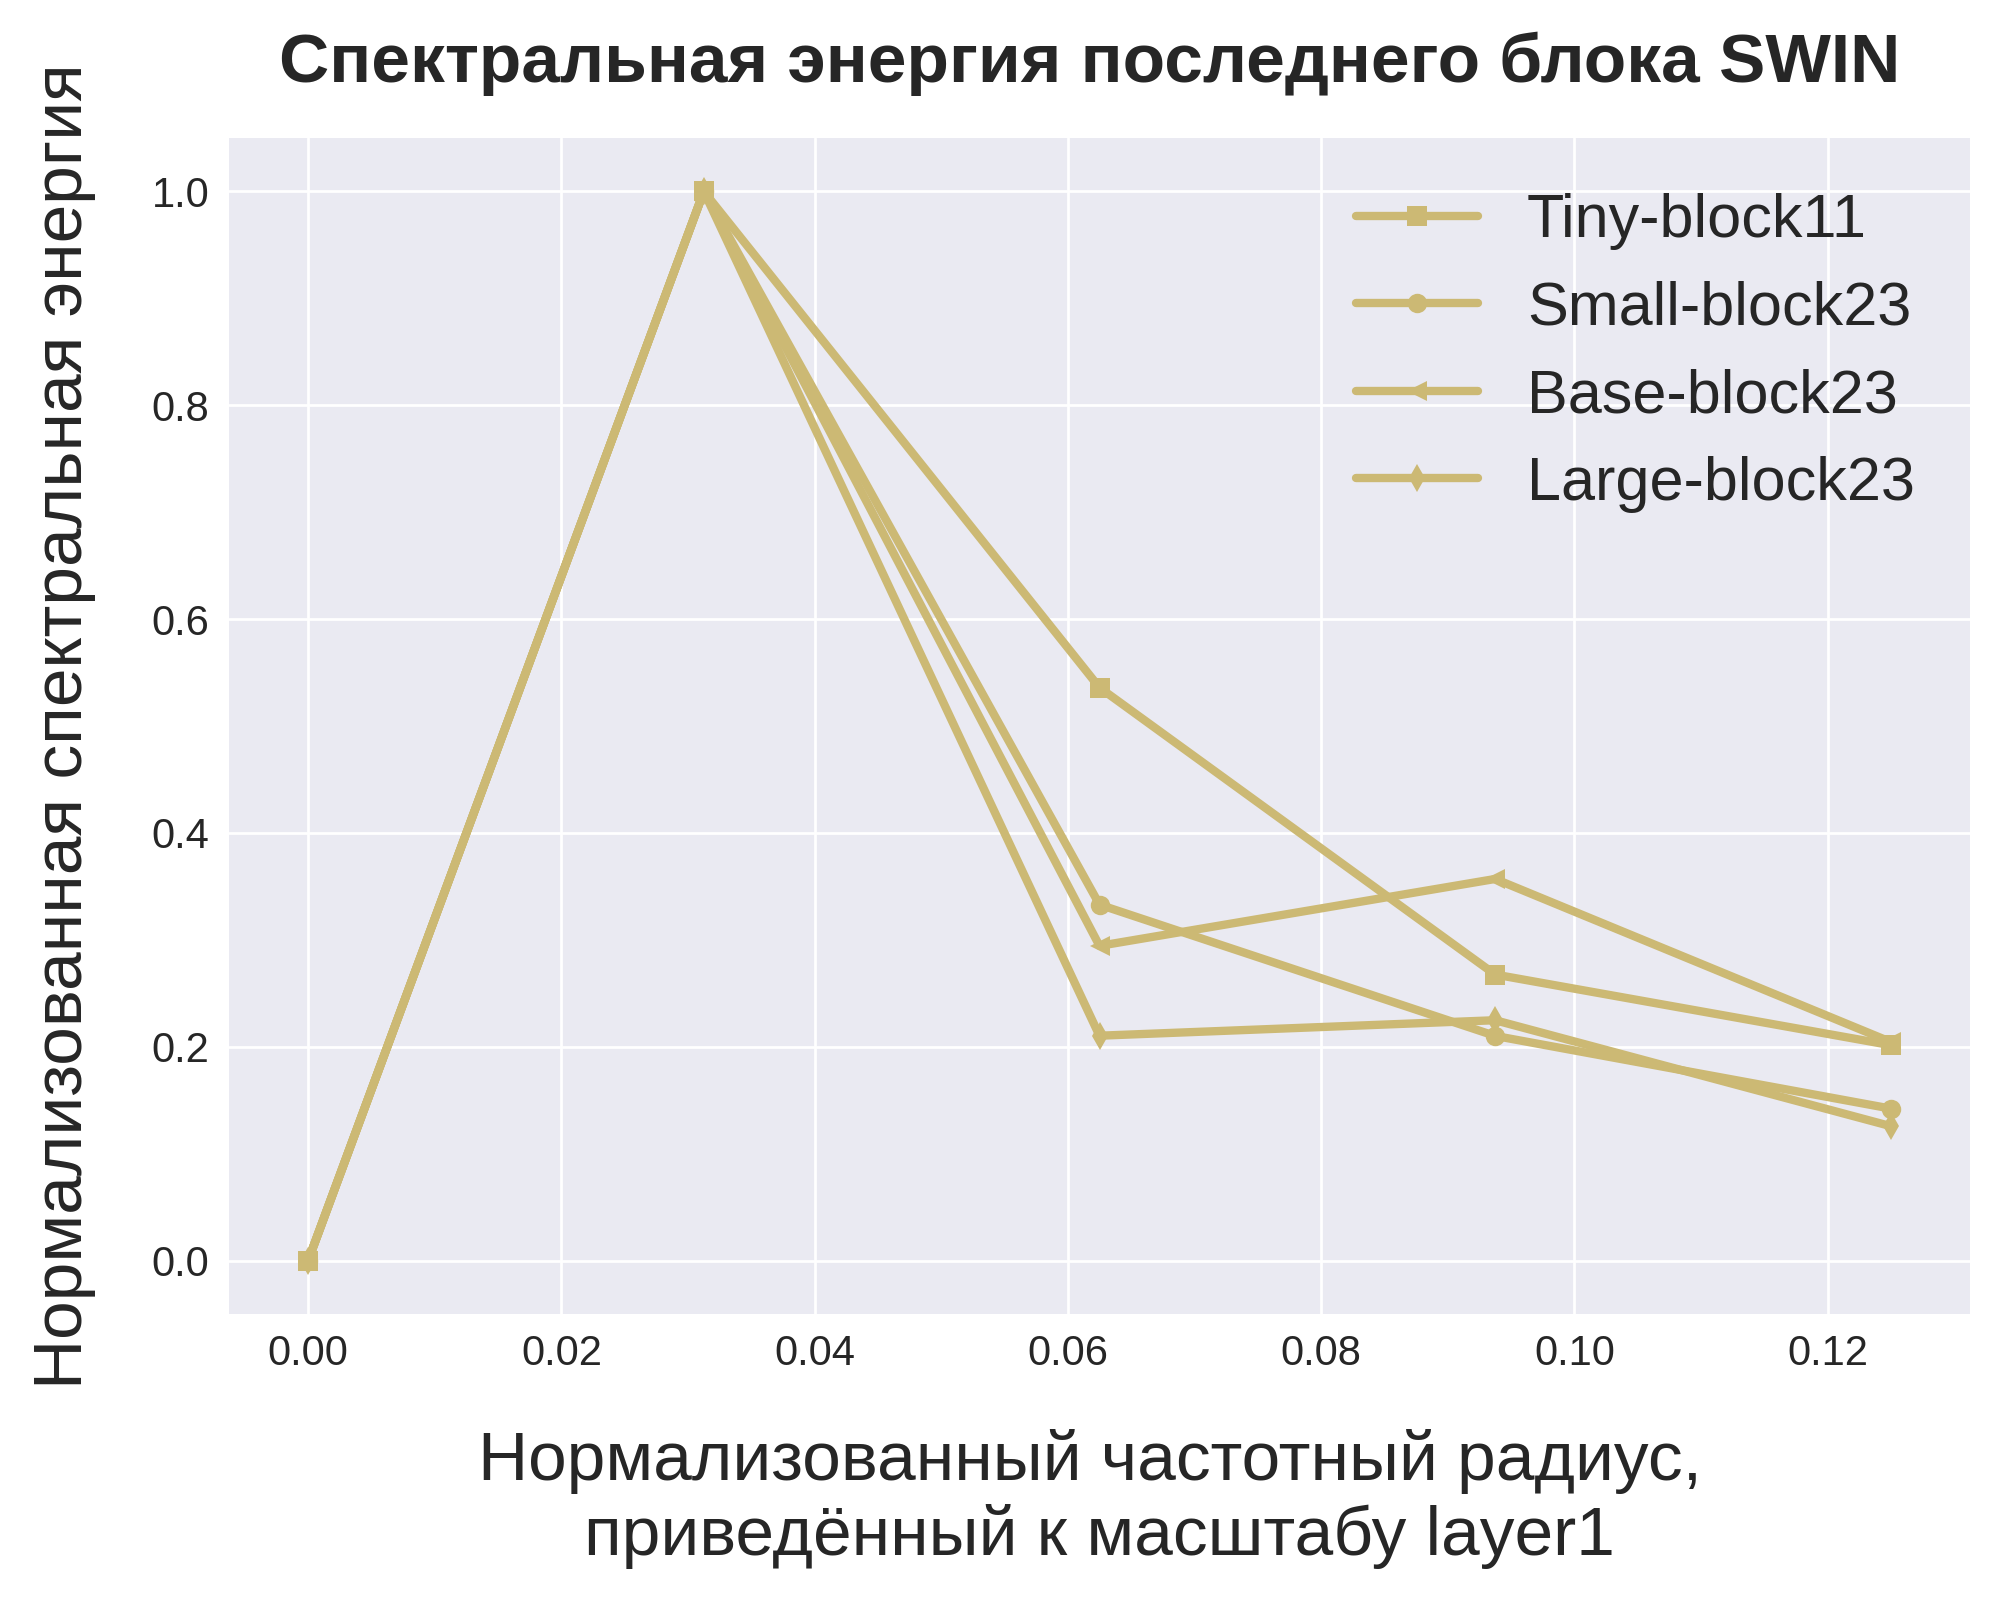
\includegraphics[width=0.8\textwidth]{images/compare/swin_block_last.png} % Масштабируем до 80% ширины текста
    \caption{Сравнение спектров последних слоёв Swin разного масштаба.} % Подпись
    \label{fig:swin_block_last} % Метка для ссылки в тексте
\end{figure}

\subsection{Межсемейственное сравнение архитектур}

На Рис. \ref{fig:compare_begin_block} показаны нормализованные радиальные спектры мощности для начальных уровней ResNet, ViT и Swin. У всех семейств максимум находится в области малых частотных радиусов. Значит, уже в начале обработки основная энергия признаков сосредоточена в низкочастотной области.

При этом кривые не совпадают. У ResNet хвост после основного пика выглядит более протяжённым: начальные свёрточные признаки ещё несут часть локальной текстурной информации. У ViT и Swin начальные представления формируются не как пиксельные карты признаков CNN, а через патчи и токены. Поэтому их спектральный профиль задаётся другой пространственной дискретизацией. На этом уровне различия между архитектурами ещё не максимальны, но видно, что каждая из них стартует с собственной формой распределения энергии.

\begin{figure}[h]
    \centering % Центрируем изображение
    
\includegraphics[width=0.8\textwidth]{images/compare/compare_begin_block.png} % Масштабируем до 80% ширины текста
    \caption{Сравнение радиальных спектров мощности начальных слоёв ResNet, ViT и Swin} % Подпись
    \label{fig:compare_begin_block} % Метка для ссылки в тексте
\end{figure}

На средних уровнях различия становятся заметнее. ResNet быстрее смещается к низкочастотной области: после пика энергия падает довольно резко, а вклад средних и высоких частот остаётся небольшим. Это хорошо согласуется с общей логикой CNN, где признаки постепенно агрегируются, рецептивное поле растёт, а пространственное разрешение уменьшается.

Сравнение средних слоёв на Рис. \ref{fig:compare_middle_block} показывает, что ViT не следует тому же сценарию. Его кривые имеют более протяжённый спад, то есть часть энергии сохраняется на средних частотах. Такая форма связана с тем, что ViT работает на решётке патчей без классического свёрточного downsampling между блоками.

Swin на этом графике ведёт себя наиболее неоднородно. Часть Swin-кривых убывает медленнее, чем ResNet, и сохраняет высокий уровень энергии в среднечастотной области. Поэтому для среднего уровня нельзя просто сказать, что Swin повторяет CNN. Скорее здесь проявляется его гибридная природа: иерархичность уже влияет на спектр, но оконное внимание и обмен между окнами дают более широкий частотный профиль.

\begin{figure}[h!]
    \centering % Центрируем изображение
    
\includegraphics[width=0.8\textwidth]{images/compare/compare_middle_block.png} % Масштабируем до 80% ширины текста
    \caption{Сравнение радиальных спектров мощности средних слоёв ResNet, ViT и Swin} % Подпись
    \label{fig:compare_middle_block} % Метка для ссылки в тексте
\end{figure}

На последних уровнях различия между семействами становятся наиболее заметными (Рис. \ref{fig:compare_last_block}). У ResNet спектры сужаются и концентрируются около малых частотных радиусов. Это соответствует финальному CNN-представлению, где локальные детали и текстурные изменения уже в основном подавлены. Дальше эту же картину подтверждают метрики: центроид у ResNet снижается, а доля низкочастотной энергии растёт.

Характер финальных кривых у архитектуры ViT принципиально иной. Ряд модификаций, в особенности масштабные конфигурации, демонстрируют выраженную хвостовую часть в среднечастотном спектре. Подобная картина контрастирует с жесткой фильтрацией низких частот, свойственной ResNet. Данное наблюдение согласуется со смещением спектрального центроида ViT в сторону более высоких значений на глубоких уровнях сети.

Финальный Swin по направлению изменения спектра ближе к CNN: диапазон становится уже, максимум остаётся около низких частот. Но полного совпадения с ResNet нет. У Swin сохраняются признаки трансформерной обработки, связанные с оконным вниманием и стадийной организацией. Поэтому его финальное поведение лучше описывать как промежуточное: низкочастотное по итоговому профилю, но сформированное другим механизмом.

\begin{figure}[h!]
    \centering % Центрируем изображение
    
\includegraphics[width=0.8\textwidth]{images/compare/compare_last_block.png} % Масштабируем до 80% ширины текста
    \caption{Сравнение радиальных спектров мощности последних слоёв ResNet, ViT и Swin} % Подпись
    \label{fig:compare_last_block} % Метка для ссылки в тексте
\end{figure}

По графикам видно, что трансформерные архитектуры не повторяют спектральную динамику CNN. ResNet даёт наиболее последовательное сжатие спектра, ViT показывает более свободное перераспределение энергии, а Swin оказывается между ними.

\section{Сводная интерпретация по метрикам}

Для численного сравнения использовались три показателя: спектральный центроид, доля низкочастотной энергии и скорость спектрального сжатия. Графики дают форму кривой, а метрики позволяют проверить те же наблюдения в компактном виде.

В Таб. \ref{tab:SpectraCentr_metrics} приведены значения спектрального центроида для моделей разных семейств. У ResNet картина самая ровная: центроид уменьшается от начальных уровней к глубоким во всех четырёх моделях. Для ResNet18 он падает с 0.176 до 0.035, для ResNet34 — с 0.169 до 0.036, для ResNet50 — с 0.203 до 0.049, для ResNet101 — с 0.206 до 0.046. Это численно подтверждает то, что было видно на графиках: по глубине ResNet сдвигает энергию к низким частотам.

Есть и небольшая деталь. У ResNet50 и ResNet101 начальный центроид выше, чем у ResNet18/34. Возможно, это связано с более широкой и сложной структурой bottleneck-блоков. Но к финальным уровням все модели приходят к близкому диапазону. Значит, более глубокая ResNet меняет траекторию сжатия, но итоговый низкочастотный характер остаётся общим для всего семейства.

\begin{table}[h]
\centering
\caption{Спектральный центроид различных архитектур} 
\label{tab:SpectraCentr_metrics}
\vspace{1ex} 
\begin{tabular}{llccc} % Добавлен один столбец 'l' слева
\toprule
\textbf{Архитектура} & \textbf{Тип} & \textbf{Начальные} & \textbf{Средние} & \textbf{Глубокие} \\
\midrule

% Первая группа строк
\multirow{4}{*}{CNN} & resnet18      & 0.176 & 0.121 & 0.035 \\
                     & resnet34      & 0.169 & 0.116 & 0.036 \\
                     & resnet50      & 0.203 & 0.128 & 0.049 \\
                     & resnet101     & 0.206 & 0.140 & 0.046 \\

\midrule

% Вторая группа строк                                                                                                       
\multirow{4}{*}{ViT} & tiny\_16      & 0.297 & 0.257 & 0.278 \\
                     & small\_16     & 0.312 & 0.419 & 0.346 \\
                     & base\_16      & 0.265 & 0.351 & 0.275 \\
                     & large\_16     & 0.275 & 0.385 & 0.437 \\
\midrule

% Третья группа строк
\multirow{4}{*}{Swin} & tiny       & 0.114 & 0.074 & 0.053 \\
                      & small      & 0.103 & 0.114 & 0.049 \\
                      & base       & 0.098 & 0.110 & 0.054 \\
                      & large      & 0.121 & 0.125 & 0.048 \\
\bottomrule
\end{tabular}
\end{table}

У ViT значения центроида выше и ведут себя менее регулярно. У ViT-large центроид растёт от 0.275 на начальном уровне до 0.437 на глубоком. У ViT-small и ViT-base максимум приходится на средний уровень: 0.419 и 0.351 соответственно. Такая динамика не похожа на устойчивое подавление средних и высоких частот. Скорее ViT перераспределяет энергию между блоками, а не просто сжимает её к низкочастотной области.

У Swin центроид в начале ниже, чем у ViT, а на глубоких блоках оказывается близок к ResNet. Финальные значения Swin лежат в диапазоне 0.048--0.054, тогда как у ResNet — 0.035--0.049. При этом средний уровень у Swin ведёт себя не полностью монотонно: у small, base и large центроид немного выше начального, у tiny — ниже. Это хорошо согласуется с графиками: Swin действительно приходит к низкочастотному финальному состоянию, но промежуточная динамика у него сложнее, чем у ResNet.

В Таб. \ref{tab:LowFrac_metrics} приведена доля низкочастотной энергии. Для CNN эта метрика растёт во всех моделях. У ResNet18 значение увеличивается с 17.3 до 31.2, у ResNet34 — с 17.8 до 31.2, у ResNet50 — с 16.6 до 30.1, у ResNet101 — с 16.3 до 30.3. Здесь центроид и доля низких частот дают согласованную картину: спектр ResNet по глубине сжимается, а низкочастотная область получает всё больший вес.

У ViT такой единой траектории нет. На начальных блоках доля низкочастотной энергии высокая: от 53.1 до 61.9. Но дальше каждая модель ведёт себя по-своему. У ViT-tiny она сначала растёт, затем падает. У ViT-small снижается на среднем уровне и частично восстанавливается на глубоком. У ViT-base после падения снова выходит на высокое значение. У ViT-large, наоборот, снижается почти монотонно — с 59.5 до 30.6. Это ещё раз показывает: ViT нельзя описать одной простой схемой низкочастотного накопления.

Высокая доля низкочастотной энергии у ViT не противоречит высокому центроиду. Эти показатели смотрят на распределение с разных сторон. Доля низких частот считает энергию ниже выбранного порога, а центроид учитывает всё распределение целиком. Поэтому возможна ситуация, когда значительная часть энергии находится у низких частот, но оставшаяся часть достаточно далеко растянута по частотной оси и поднимает центроид. Для ViT такая комбинация как раз и характерна.

У Swin доля низких частот к глубоким блокам растёт во всех вариантах. Начальные значения находятся около 21.5--22.6, глубокие — около 29.5--29.9. На среднем уровне изменения небольшие и не всегда направлены одинаково, но финальный переход к низкочастотному представлению сохраняется. В этом смысле Swin ближе к ResNet, чем к ViT, хотя степень и форма сжатия у него другие.

\begin{table}[h]
\centering
\caption{Доля низкочастотной энергии различных архитектур} 
\label{tab:LowFrac_metrics}
\vspace{1ex} 
\begin{tabular}{llccc} % Добавлен один столбец 'l' слева
\toprule
\textbf{Архитектура} & \textbf{Тип} & \textbf{Начальные} & \textbf{Средние} & \textbf{Глубокие} \\
\midrule

% Первая группа строк
\multirow{4}{*}{CNN} & resnet18      & 17.3 & 21.0 & 31.2 \\
                     & resnet34      & 17.8 & 21.6 & 31.2 \\
                     & resnet50      & 16.6 & 20.3 & 30.1 \\
                     & resnet101     & 16.3 & 19.2 & 30.3 \\

\midrule

% Вторая группа строк                                                                                                   
\multirow{4}{*}{ViT} & tiny\_16      & 55.6 & 63.5 & 44.7 \\
                     & small\_16     & 53.1 & 32.8 & 47.3 \\
                     & base\_16      & 61.9 & 47.0 & 62.5 \\
                     & large\_16     & 59.5 & 40.3 & 30.6 \\
\midrule

% Третья группа строк
\multirow{4}{*}{Swin} & tiny       & 21.8 & 25.9 & 29.6 \\
                      & small      & 22.4 & 22.2 & 29.9 \\
                      & base       & 22.6 & 22.6 & 29.5 \\
                      & large      & 21.5 & 21.3 & 29.9 \\
\bottomrule
\end{tabular}
\end{table}

Таб. \ref{tab:models_metrics} показывает скорость спектрального сжатия. У CNN все значения положительные и большие: от 0.46 до 0.51. Это самый выраженный режим сжатия среди трёх семейств. У ViT значения близки к нулю или отрицательны: от -0.0 до -0.12. По выбранной метрике это означает отсутствие устойчивого движения к низкочастотному представлению. У Swin значения положительные, но заметно меньше, чем у CNN: от 0.04 до 0.16. Значит, Swin всё же сжимает спектр к глубоким блокам, но делает это мягче.

\begin{table}[h]
\centering
\caption{Скорость спектрального сжатия} 
\label{tab:models_metrics}
\vspace{1ex} 

\begin{tabular}{ccccc} 
\toprule
\textbf{Архитектура} & \textbf{Tiny(18)} & \textbf{Small(34)} & \textbf{Base(50)} & \textbf{Large(101)} \\
\midrule
CNN    & 0.48 & 0.46  & 0.50  & 0.51 \\
ViT    & -0.0 & -0.05 & -0.02 & -0.12 \\
SWIN   & 0.16 & 0.07  & 0.04  & 0.12 \\
\bottomrule
\end{tabular}
\end{table}

Сопоставление трёх таблиц даёт общий вывод по метрикам. Тип архитектуры влияет на спектральную динамику сильнее, чем размер модели внутри одного семейства. Все ResNet демонстрируют сжатие, все Swin приходят к низкочастотному финальному профилю, но с меньшей скоростью, а ViT показывает наиболее нестабильную и немонотонную динамику. Это согласуется с визуальным анализом спектральных кривых.

\section{Обобщение экспериментальных результатов}

Совместный анализ графиков и таблиц показывает, что архитектуры различаются не только точностью или числом параметров. Они по-разному меняют частотный состав внутренних представлений. Это видно уже на уровне спектральных кривых, а затем подтверждается центроидом, долей низких частот и скоростью сжатия.

Для ResNet наблюдается самый понятный сценарий. Центроид падает, доля низкочастотной энергии растёт, скорость сжатия положительна во всех вариантах. Иначе говоря, ResNet последовательно переводит представления от более детальных пространственных признаков к сглаженным и семантически более крупным структурам. Это соответствует устройству CNN: свёртки, downsampling и рост рецептивного поля работают в одном направлении.

ViT ведёт себя иначе. Его центроид может расти на средних или поздних блоках, а доля низких частот меняется без единого шаблона. Это не случайная мелочь, а характерная особенность архитектуры: изображение обрабатывается как последовательность патчей, и блоки внимания вместе с MLP и residual-соединениями не обязаны давать монотонное спектральное сжатие. Поэтому ViT в данной постановке лучше описывать как модель с немонотонным перераспределением энергии по частотной оси.

Swin занимает промежуточное место. На глубоких блоках он приходит к низким значениям центроида и высокой доле низкочастотной энергии, то есть финально сближается с CNN. Но на средних уровнях у части моделей наблюдается менее прямой ход кривых и метрик. Возможно, это связано с тем, что Swin объединяет иерархию и patch merging с оконным вниманием. По результатам его нельзя назвать простой копией ResNet; это отдельный режим спектральной динамики.

Если сопоставить спектральные характеристики с точностью классификации, простой линейной зависимости не получается. Более сильное сжатие не всегда означает лучшую модель, а более широкий спектр не гарантирует более высокое качество. Спектральные метрики здесь работают иначе: они помогают понять, как устроены внутренние представления, но не заменяют accuracy.

Главный экспериментальный результат можно сформулировать так: ResNet даёт последовательное низкочастотное сжатие, ViT — немонотонное перераспределение спектральной энергии, Swin — промежуточную динамику с финальным смещением к низким частотам. Архитектура оказывается главным фактором, задающим форму этого поведения.


% \begin{table}[h]
% \centering
% \caption{Точность предсказаний} 
% \label{tab:models_metrics}
% \vspace{1ex} 

% \begin{tabular}{ссccc} 
% \toprule
% \textbf{Архитектура} & \textbf{Tiny(18)} & \textbf{Small(34)} & \textbf{Base(50)} & \textbf{Large(101)} \\
% \midrule
% CNN    &  79.04  &  85.36  &  92.89  &  93.96 \\
% ViT    &  82.10  &  87.96  &  92.02  &  92.28 \\
% SWIN   &  88.19  &  91.59  &  92.25  &  93.03 \\
% \bottomrule
% \end{tabular}
% \end{table}
